\whiteBGstarBegin

\begin{enumerate}[label=\bfseries Câu \arabic*:]
	
	\item \mkstar{1}
	
	\cauhoi{Tính cường độ điện trường do một điện tích điểm $4\cdot 10^{-9}\ \text{C}$ gây ra tại một điểm cách nó $\SI{5}{cm}$ trong chân không
		
		\begin{mcq}(4)
			\item $\SI{144}{kV/m}$.
			\item $\SI{14.4}{kV/m}$.
			\item $\SI{288}{kV/m}$.
			\item $\SI{28.8}{kV/m}$.
		\end{mcq}
	}
	
	\loigiai{\textbf{Đáp án: B.}
		
		Áp dụng công thức tính cường độ điện trường:
		\begin{equation*}
			E = k\dfrac{|Q|}{\varepsilon r^2} = \text{14,4} \cdot 10^3\ \text{V/m}.
		\end{equation*}
		
		
	}
	\item \mkstar{1}
	
	\cauhoi{Một điện tích điểm $q = 4\cdot 10^{-8}\ \text{C}$ được đặt trong môi trường dầu hỏa có hằng số điện môi $\varepsilon= 2$. Độ lớn cường độ điện trường do điện tích $q$ gây ra tại điểm M cách điện tích đoạn $R = 5\ \text{cm}$ bằng
		
		\begin{mcq}(4)
			\item $\SI{72000}{V}$.
			\item $\SI{144000}{V/m}$.
			\item $\SI{72000}{V/m}$.
			\item $\SI{7.2}{V/m}$.
		\end{mcq}
	}
	
	\loigiai{\textbf{Đáp án: C.}
		
		Cường độ điện trường do điện tích $q$ gây ra tại M:
		
		\begin{equation*}
			E = k\dfrac{|q|}{\varepsilon R^2} = 72000\ \text{V/m}.
		\end{equation*}	
		
		
	}
	\item \mkstar{1}
	
	\cauhoi{Một điện tích điểm $q= -2 \cdot 10^{-7}\ \text{C}$, đặt tại điểm A trong môi trường có hằng số điện môi $\varepsilon= 2$. Véc tơ cường độ điện trường do điện tích O gây ra tại điểm B với $\text{AB} = \SI{7.5}{cm}$ có
		
		\begin{mcq}
			\item phương AB, chiều từ A đến B, độ lớn $\text{2,5}\cdot 10^5$ V/m.
			\item phương AB, chiều từ B đến A, độ lớn $\text{1,6}\cdot 10^5$ V/m.
			\item phương AB, chiều từ B đến A, độ lớn $\text{2,5}\cdot 10^5$ V/m.
			\item phương AB, chiều từ A đến B, độ lớn $\text{1,6}\cdot 10^5$ V/m.
		\end{mcq}
	}
	
	\loigiai{\textbf{Đáp án: B.}
		
		Vì $q$ là điện tích âm nên chiều của điện trường hướng về A.
		
		Áp dụng công thức tính cường độ điện trường:
		
		\begin{equation*}
			E = k\dfrac{|q|}{\varepsilon r^2} = \text{160} \cdot 10^3\ \text{V/m}.
		\end{equation*}
		
		
	}
		\item \mkstar{1}
	
	\cauhoi{Tìm phát biểu \textbf{sai}.
		\begin{mcq}
			\item Thế năng của điện tích $q$ đặt tại điểm M trong điện trường đặc trưng cho khả năng sinh công của điện trường tại điểm đó.
			\item Thế năng của điện tích $q$ đặt tại điểm M trong điện trường $W_\text{M} = q\cdot V_\text{M}$.
			\item Công của lực điện bằng độ giảm thế năng của điện tích trong điện trường.
			\item Thế năng của điện tích $q$ đặt tại điểm M trong điện trường không phụ thuộc điện tích $q$.
		\end{mcq}
	}
	
	\loigiai{\textbf{Đáp án: D.}
		
		Thế năng của một điện tích q tại điểm M trong điện trường:
		\begin{equation*}
			W_\text{M} = A_{\text{M}\infty} =qV_\text{M}
		\end{equation*}
		Thế năng tỉ lệ thuận với $q$. Độ lớn và dấu của thế năng phụ thuộc vào cách chọn gốc thế năng.
		
		
	}
	
	\item \mkstar{1}
	
	\cauhoi{Công của lực điện trong sự di chuyển của điện tích $q$ trong điện trường từ điểm M đến điểm N \textbf{không} phụ thuộc vào yếu tố nào sau đây?
		\begin{mcq}
			\item Độ lớn của cường độ điện trường.
			\item Hình dạng đường đi từ điểm M đến điểm N.
			\item Điện tích $q$.
			\item Vị trí của điểm M và điểm N.
		\end{mcq}
	}
	
	\loigiai{\textbf{Đáp án: B.}
		
		Công của lực điện tác dụng lên điện tích không phụ thuộc vào hình dạng đường đi của điện tích mà chỉ phụ thuộc vào điểm đầu và điểm cuối của đường đi trong điện trường, do đó người ta nói điện trường tĩnh là một trường thế.
		
		
	}
	\item \mkstar{1}
	
	\cauhoi{Một điện tích $q$ chuyển động trong điện trường không đều theo một đường cong kín. Gọi công của lực điện trong chuyển động đó là $A$ thì
		\begin{mcq}
			\item $A > 0$ nếu $q > 0$.
			\item $A > 0$ nếu $q < 0$.
			\item $A \neq 0$ còn dấu của $A$ chưa xác định vì chưa biết chiều chuyển động của $q$.
			\item $A = 0$ trong mọi trường hợp.
		\end{mcq}
	}
	
	\loigiai{\textbf{Đáp án: D.}
		
		Vì điện tích chuyển động trên đường cong kín thì lực điện không sinh công.
		
		
	}
	\item \mkstar{1}

\cauhoi{Hai điểm M, N nằm trên cùng một đường sức của một điện trường đều, hiệu điện thế giữa M, N là $U_\text{MN}$. Công thức nào sau đây đúng?
	\begin{mcq}(2)
		\item $U_\text{MN}= U_\text{NM}$.
		\item $U_\text{MN}=V_\text{M} - V_\text{N}$.
		\item $U_\text{MN}=V_\text{N} - V_\text{M}$.
		\item $A=\dfrac{q}{U_\text{MN}}$.
	\end{mcq}
}

\loigiai{\textbf{Đáp án: B.}
	
	Hiệu điện thế giữa M và N có công thức 
	\begin{equation*}
		U_\text{MN}=V_\text{M} - V_\text{N}
	\end{equation*}
	
	
}

\item \mkstar{1}

\cauhoi{Hãy cho biết mối liên hệ giữa hiệu điện thế giữa hai điểm M, N.
	
	\begin{mcq}(2)
		\item $U_\text{MN}>U_\text{NM}$.
		\item $U_\text{MN} < U_\text{NM}$.
		\item $U_\text{MN}= U_\text{NM}$.
		\item $U_\text{MN}=-U_\text{NM}$.
	\end{mcq}
}

\loigiai{\textbf{Đáp án: D.}
	
	Ta có:
	
	\begin{equation*}
		U_\text{MN}=V_\text{M} - V_\text{N} 
	\end{equation*}
	\begin{equation*}
		U_\text{NM}=V_\text{N} - V_\text{M} 
	\end{equation*}
	Suy ra 
	\begin{equation*}
		U_\text{MN}= - U_\text{NM}.
	\end{equation*}
	
	
	
}
	\item \mkstar{2}
	
	\cauhoi{Một quả cầu kim loại bán kính $\SI{4}{cm}$ mang điện tích $q = 5\cdot 10^{-8}\ \text{C}$. Tính cường độ điện trường tại điểm M cách tâm quả cầu $\SI{10}{cm}$.
		\begin{mcq}(4)
			\item 1,9$\cdot 10^5$ V/m.
			\item 2,8$\cdot 10^5$ V/m.
			\item 3,6$\cdot 10^5$ V/m.	
			\item 0,45$\cdot 10^5$ V/m.
		\end{mcq}
	}
	
	\loigiai{\textbf{Đáp án: D.}
		
		Lưu ý: Không trừ bán kính quả cầu vì khi xét một quả cầu mang điện tích, toàn bộ điện tích được xem như một điện tích điểm nằm tại tâm quả cầu.
		
		Cường độ điện trường tại M là:
		
		\begin{equation*}
			E = k\dfrac{|q|}{R^2} = 45000\ \text{V/m}.
		\end{equation*}
		
		
	}
	
	\item \mkstar{2}
	
	\cauhoi{Điện trường trong khí quyển gần mặt đất có cường độ $\SI{200}{V/m}$, hướng thẳng đứng từ trên xuống dưới. Một positron ($+e = +\text{l,6}\cdot 10^{-19}\ \text{C}$) ở trong điện trường này sẽ chịu tác dụng một lực điện có cường độ và hướng như thế nào?
		\begin{mcq}
			\item 3,2$\cdot 10^{-21}$ N, hướng thẳng đứng từ trên xuống.
			\item 3,2$\cdot 10^{-21}$ N, hướng thẳng đứng từ dưới lên.
			\item 3,2$\cdot 10^{-17}$ N, hướng thẳng đứng từ trên xuống.
			\item 3,2$\cdot 10^{-17}$ N, hướng thẳng đứng từ dưới lên.
		\end{mcq}
	}
	
	\loigiai{\textbf{Đáp án: C.}	
		
		Do điện tích dương nên lực điện sẽ cùng chiều với cường độ điện trường: hướng thẳng đứng từ trên xuống.
		
		Lực điện có độ lớn:
		
		\begin{equation*}
			F = qE = \text{3,2} \cdot 10^{-17}\ \text{N}.
		\end{equation*}
		
		
	}
	
	\item \mkstar{2}
	
	\cauhoi{Điện tích điểm $q = -3\ \mu \text{C}$ đặt tại điểm có cường độ điện trường $E = 12000\ \text{V/m}$, có phương thẳng đứng chiều từ trên xuống dưới. Xác định phương chiều và độ lớn của lực tác dụng lên điện tích $q$.
		\begin{mcq}
			\item $\vec {F}$ có phương thẳng đứng, chiều từ trên xuống dưới, $F = \text{0,36}\ \text{N}$.
			\item $\vec {F}$ có phương nằm ngang, chiều từ trái sang phải, $F = \text{0,48}\ \text{N}$.
			\item $\vec {F}$ có phương thẳng đứng, chiều từ dưới lên trên, $F = \text{0,36}\ \text{N}$.
			\item $\vec {F}$ có phương thẳng đứng, chiều từ dưới lên trên, $F = \text{0,036}\ \text{N}$.
		\end{mcq}
	}
	
	\loigiai{\textbf{Đáp án: D.}
		
		Ta có: 
		\begin{equation*}
			\vec{F} =q \vec{E} \Rightarrow F =|q|E = \text{0,036}\ \text{N}.
		\end{equation*}
		Do $q<0$ nên lực $\vec{F}$ có phương thẳng đứng chiều ngược với chiều của $\vec{E}$.
		
		Vậy $F = \text{0,036} \ \text{N}$, có phương thẳng đứng, chiều hướng từ dưới lên trên.
		
		
	}
	\item \mkstar{2}
	
	\cauhoi{Đáp án nào là đúng khi nói về quan hệ về hướng giữa véctơ cường độ điện trường và lực điện trường?
		\begin{mcq}
			\item $\vec E$ cùng phương chiều với $\vec F$ tác dụng lên điện tích thử đặt trong điện trường đó.
			\item $\vec E$ cùng phương ngược chiều với $\vec F$ tác dụng lên điện tích thử đặt trong điện trường đó.
			\item $\vec E$ cùng phương chiều với $\vec F$ tác dụng lên điện tích thử dương đặt trong điện trường đó.
			\item $\vec E$  cùng phương chiều với $\vec F$ tác dụng lên điện tích thử âm đặt trong điện trường đó.
		\end{mcq}
	}
	
	\loigiai{\textbf{Đáp án: C.}
		
		Cường độ điện trường $\vec {E} = \dfrac{\vec{F}}{q} \Rightarrow \vec{E}\cdot \vec{F}$.
		
		Chiều của $\vec E$ thì phụ thuộc vào dấu của điện tích thử $q$.
		
		$q$ dương: $\vec E, \vec F$ cùng chiều.
		
		$q$ âm: $\vec E, \vec F$ ngược chiều.
		
		
	}
	\item \mkstar{2}
	
	\cauhoi{Một điện tích $q = 10^{-7}\ \text{C}$ đặt trong điện trường của một điện tích điểm $Q$, chịu tác dụng lực $F = 3\ \text{mN}$. Tính độ lớn của điện tích $Q$. Biết rằng hai điện tích cách nhau một khoảng $r = 30\ \text{cm}$ trong chân không.
		\begin{mcq}(4)
			\item 0,5 $\mu$C.
			\item 0,3 $\mu$C.
			\item 0,4 $\mu$C.
			\item 0,2 $\mu$C.
		\end{mcq}
	}
	
	\loigiai{\textbf{Đáp án: B.}
		
		Cường độ điện trường
		\begin{equation*}
			E =\dfrac{F}{|q|} = 3 \cdot 10^7\ \text{V/m}.
		\end{equation*}
		Ta lại có:
		\begin{equation*}
			E =k\dfrac{|Q|}{r^2} \Rightarrow |Q| = \dfrac{Er^2}{k} = 3 \cdot 10^{-7}\ \text{C}.
		\end{equation*}
		
		
	}
	\item \mkstar{2}
	
	\cauhoi{Cường độ điện trường do điện tích $+Q$ gây ra tại điểm A cách nó một khoảng $r$ có độ lớn là $E$. Nếu thay bằng điện tích $-2Q$ và giảm khoảng cách đến A còn một nửa thì cường độ điện trường tại A có độ lớn là
		\begin{mcq}(4)
			\item $8E$.
			\item $4E$.
			\item $\text{0,25}E$.
			\item $E$.
		\end{mcq}
	}
	
	\loigiai{\textbf{Đáp án: A.}
		
		Ban đầu
		\begin{equation*}
			E = k \dfrac{|Q|}{\varepsilon r^2}.
		\end{equation*}
		Khi thay bằng điện tích $-2Q; r'=\dfrac{r}{2}$, ta có:
		\begin{equation*}
			E'=k\dfrac{|-2Q|}{\left(\dfrac{r'}{2}\right)^2} = 8E.
		\end{equation*}
		
		
	}
	\item \mkstar{2}
	
	\cauhoi{Cường độ điện trường của một điện tích điểm tại A bằng $\SI{36}{V/m}$, tại B bằng $\SI{9}{V/m}$. Hỏi cường độ điện trường tại trung điểm C của AB bằng bao nhiêu, biết hai điểm A, B nằm trên cùng một đường sức?
		\begin{mcq}(4)
			\item $\SI{30}{V/m}$.
			\item $\SI{25}{V/m}$.
			\item $\SI{16}{V/m}$.
			\item $\SI{12}{V/m}$.
		\end{mcq}
	}
	
	\loigiai{\textbf{Đáp án: C.}
		
		Công thức tính cường độ điện trường
		\begin{equation*}
			E = k \dfrac{|q|}{r^2}.
		\end{equation*}
		Ta suy ra được 
		\begin{equation*}
			r \sim  \dfrac{1}{\sqrt E}.
		\end{equation*}
		Mà: 
		\begin{equation*}
			r_\text{C} =\dfrac{r_\text{A} + r_\text{B}}{2}.
		\end{equation*}
		Vậy 
		\begin{equation*}
			\dfrac{1}{\sqrt {E_\text{C}}} = \dfrac{1}{2} \left (\dfrac{1}{\sqrt {E_\text{A}}}+ \dfrac{1}{\sqrt{E_\text{B}}}\right) \Rightarrow E_\text{C} = 16\ \text{V/m}
		\end{equation*}
		
	}
	\item \mkstar{2}
	
	\cauhoi{Cường độ điện trường tạo bởi một điện tích điểm cách nó $\SI{2}{cm}$ bằng $10^5$ V/m. Tại vị trí cách điện tích này bằng bao nhiêu thì cường độ điện trường bằng $4\cdot 10^5$ V/m? 
		\begin{mcq}(4)
			\item $\SI{2}{cm}$.
			\item $\SI{1}{cm}$.
			\item $\SI{4}{cm}$.
			\item $\SI{5}{cm}$.
		\end{mcq}
	}
	
	\loigiai{\textbf{Đáp án: B.}
		
		Tại vị trí cách điện tích điểm $Q$ khoảng $r = 2\ \text{cm}$:
		\begin{equation*}
			E_1= k\dfrac{|Q|}{\varepsilon r_1} = 10^5\ \text{V/m}.
		\end{equation*}
		Gọi $r'$ là vị trí cách điện tích để cường độ điện trường $E_2 = 4\cdot 10^5$ V/m. Ta có:
		\begin{equation*}
			E_2= k\dfrac{|Q|}{\varepsilon r_2} = 4\cdot 10^5\ \text{V/m}.
		\end{equation*}
		Lập tỉ số :
		\begin{equation*}
			\dfrac{E_1}{E_2} = \dfrac{r'^2}{r^2} \Rightarrow r' = r \sqrt{\dfrac{10^5}{4\cdot 10^5}} = 1\ \text{cm}. 
		\end{equation*}
		
	}
	
		\item \mkstar{2}
	
	\cauhoi{Công của lực điện trường dịch chuyển một điện tích $-2\ \mu \text{C}$ từ A đến B là $\SI{4}{mJ}$. $U_\text{AB}$ bằng
		\begin{mcq}(4)
			\item $\SI{2}{V}$.
			\item $\SI{2000}{V}$.
			\item $\SI{-8}{V}$.
			\item $\SI{-2000}{V}$.
		\end{mcq}
	}
	
	\loigiai{\textbf{Đáp án: D.}	
		
		Ta có:
		\begin{equation*}
			U_\text{AB} =\dfrac{A_\text{AB}}{q} = - 2000\ \text{V}.
		\end{equation*}
		
		
		
	}
	\item \mkstar{2}
	
	\cauhoi{Một điện tích điểm $q = -2\cdot 10^{-7}\ \text{C}$ di chuyển được đoạn đường $\SI{5}{cm}$ dọc theo một đường sức của điện trường đều có cường độ điện trường $\SI{5000}{V/m}$. Công của lực điện thực hiện trong quá trình di chuyển của điện tích $q$ là
		\begin{mcq}(4)
			\item $-5\cdot 10^{-5}\ \text{J}$.
			\item $5\cdot 10^{-5}\ \text{J}$.
			\item $5\cdot 10^{-3}\ \text{J}$.
			\item $-5\cdot 10^{-3}\ \text{J}$.
		\end{mcq}
	}
	
	\loigiai{\textbf{Đáp án: A.}
		
		Ta có: $q$ là điện tích âm, $q$ di chuyển được đoạn đường 5 cm dọc theo một đường sức điện nên $d = \SI{0.05}{m}$ ($d > 0$).
		
		\begin{equation*}
			A = qEd = -5 \cdot 10^{-5}\ \text{J}
		\end{equation*}
		
		
	}
	\item \mkstar{2}
	
	\cauhoi{Một điện tích điểm q di chuyển trong một điện trường từ điểm C đến điểm D thì lực điện sinh công $\SI{1.2}{J}$. Nếu thế năng của điện tích $q$ tại D là $\SI{0.4}{J}$ thì thế năng của nó tại C là
		\begin{mcq}(4)
			\item $\SI{-1.6}{J}$.
			\item $\SI{1.6}{J}$.
			\item $\SI{0.8}{J}$.
			\item $\SI{-0.8}{J}$.
		\end{mcq}
	}
	
	\loigiai{\textbf{Đáp án: B.}
		
		Ta có:
		\begin{equation*}
			A_\text{CD} =W_\text{C} - W_\text{D} \Rightarrow W_\text{C} = A_\text{CD} + W_\text{D} = \text{1,6}\ \text{J}.
		\end{equation*}
		
		
	}
	\item \mkstar{2}
	
	\cauhoi{Điện tích điểm $q = -3\cdot 10^{-6}\ \text{C}$ di chuyển được đoạn đường $\SI{2.5}{cm}$ dọc theo một đường sức điện nhưng ngược chiều của đường sức trong một điện trường đều có cường độ điện trường $\SI{4000}{V/m}$. Công của lực điện trong sự di chuyển của điện tích $q$ là
		\begin{mcq}(4)
			\item $3\cdot 10^{-4}\ \text{J}$.
			\item $-3\cdot 10^{-4}\ \text{J}$.
			\item $3\cdot 10^{-2}\ \text{J}$.
			\item $-3\cdot 10^{-3}\ \text{J}$.
		\end{mcq}
	}
	
	\loigiai{\textbf{Đáp án: A.}
		
		$q$ là điện tích âm, $q$ di chuyển được đoạn đường $\SI{5}{cm}$ dọc theo một đường sức điện nhưng ngược chiều đường sức nên $d < 0$, $d=\SI{- 0.025}{m}$.
		
		Ta có:
		\begin{equation*}
			A = qEd = 3 \cdot 10^{-4}\ \text{J}.
		\end{equation*}
		
		
	}
	\item \mkstar{2}
	
	\cauhoi{Công của lực điện trường dịch chuyển một điện tích $4\ \mu \text{C}$ dọc theo chiều một đường sức trong một điện trường đều $\SI{1000}{V/m}$ trên quãng đường dài $\SI{1}{m}$ là
		\begin{mcq}(4)
			\item $\SI{4000}{J}$.
			\item $\SI{4}{J}$.
			\item $\SI{4}{mJ}$.
			\item 4 $\mu$ J.
		\end{mcq}
	}
	
	\loigiai{\textbf{Đáp án: C.}
		
		Công của lực điện trường
		\begin{equation*}
			A = qEd = 4 \cdot 10^{-3}\ \text{J} = 4\ \text{mJ}.
		\end{equation*}
		
		
	}
	\item \mkstar{2}
	
	\cauhoi{Cho điện tích $q = + 10^{-8}\ \text{C}$ dịch chuyển giữa 2 điểm cố định trong một điện trường đều thì công của lực điện trường là $\SI{60}{mJ}$. Nếu một điện điện tích $q’ = + 4\cdot 10^{-9}\ \text{C}$ dịch chuyển giữa hai điểm đó thì công của lực điện trường khi đó là
		\begin{mcq}(4)
			\item $\SI{24}{mJ}$.
			\item $\SI{20}{mJ}$.
			\item $\SI{240}{mJ}$.
			\item $\SI{120}{mJ}$.
		\end{mcq}
	}
	
	\loigiai{\textbf{Đáp án: A.}
		
		Ta có:
		\begin{equation*}
			A = qEd 
		\end{equation*}
		Lập tỉ số 
		\begin{equation*}
			\dfrac{A}{A'} = \dfrac{q}{q'} \Rightarrow A' = \text{0,4}A =24\ \text{mJ}.
		\end{equation*}
		
		
		
	}
	\item \mkstar{2}
	
	\cauhoi{Cho điện tích $q = +10^{-8}\ \text{C}$ dịch chuyển giữa 2 điểm cố định trong một điện trường đều thì công của lực điện trường là $\SI{90}{mJ}$. Nếu một điện điện tích $q’ = + 4\cdot 10^{-9}\ \text{C}$ dịch chuyển giữa hai điểm đó thì công của lực điện trường khi đó là
		\begin{mcq}(4)
			\item $\SI{225}{mJ}$.
			\item $\SI{20}{mJ}$.
			\item $\SI{36}{mJ}$.
			\item $\SI{120}{mJ}$.
		\end{mcq}
	}
	
	\loigiai{\textbf{Đáp án: C.}
		
		Ta có: 
		\begin{equation*}
			A_1 = q_1Ed; A_2 = q_2Ed.
		\end{equation*}
		\begin{equation*}
			\dfrac{A_1}{A_2} =\dfrac{q_1}{q_2} \Rightarrow A_2 =36\ \text{mJ}.
		\end{equation*}
		
		
		
	}
	\item \mkstar{2}
	
	\cauhoi{Khi điện tích dịch chuyển trong điện trường đều theo chiều đường sức thì nó nhận được một công $\SI{20}{J}$. Khi dịch chuyển theo hướng tạo với hướng đường sức $60^\circ$ trên cùng độ dài quãng đường thì nó nhận được một công là
		\begin{mcq}(4)
			\item 10 J.
			\item $5\sqrt 3$ J.
			\item $10\sqrt 2$ J.
			\item 15 J.
		\end{mcq}
	}
	
	\loigiai{\textbf{Đáp án: A.}
		
		Ta có: 
		\begin{equation*}
			A_1 = qEd; A_2 = qEd\cos 60^\circ.
		\end{equation*}
		Lập tỉ số. 
		Ta có: 
		\begin{equation*}
			\dfrac{A_1}{A_2} =\dfrac{1}{\cos 60^\circ} =2 \Rightarrow A_2 = 10\ \text{J}.
		\end{equation*}
		
		
		
		
	}

	\item \mkstar{3}
	
	\cauhoi{Tại hai điểm A, B trong chân không có hai điện tích điểm $q_1 =16 \cdot 10^{-10}\ \text{C}$  và $q_2 =-9 \cdot 10^{-10}\ \text{C}$. Độ lớn cường độ điện trường tổng hợp tại điểm C nằm cách A đoạn 4 cm, cách B đoạn 3 cm bằng bao nhiêu? Biết $AB = 5\ \text{cm}$. 
		\begin{mcq}(4)
			\item 9000 V/m.
			\item 18000 V/m.
			\item 9000$\sqrt2$ V/m.
			\item 0,9 $\sqrt2$ V/m.
		\end{mcq}
	}
	
	\loigiai{\textbf{Đáp án: C.}
		
		Nhận thấy AB$^2 =$ AC$^2$ + CB$^2$ = $5^2$ suy ra tam giác ABC vuông tại C.
		
		Gọi $\vec{E}_1, \vec{E}_2$ lần lượt là cường độ điện trường do điện tích $q_1$ và $q_2$ gây ra tại C. 
		
		Ta có:
		
		\begin{equation*}
			E_1 = k \dfrac{|q_1|}{r^2_1} = k \dfrac{|q_1|}{\text{AC}^2} = 9000\ \text{V/m}.
		\end{equation*}
		\begin{equation*}
			E_2 = k \dfrac{|q_1|}{r^2_2} = k \dfrac{|q_1|}{\text{CB}^2} = 9000\ \text{V/m}.
		\end{equation*}
		Ta có:
		\begin{equation*}
			\vec{E} = \vec{E_1}+\vec{E_2}.
		\end{equation*}
		Vì $\vec{E_1}$ vuông góc $\vec{E_2}$.
		
		Suy ra $E = \sqrt {E_1^2+E_2^2} = 9000\sqrt 2\ \text{V/m}$.
		
		
	}
	\item \mkstar{3}
	
	\cauhoi{Cho hai điện tích $q_1 =1\ \text{nC}, q_2 =3\ \text{nC}$ đặt tại hai điểm A, B theo thứ tự đó trong chân không cách nhau một khoảng AB = 60 cm. Tìm điểm C mà cường độ điện trường tại đó do điện tích $q_1$ gây ra liên hệ với cường độ điện trường do $q_2$ gây ra theo hệ thức $\vec{E}_1 =-3 \vec{E}_2$.
		\begin{mcq}(2)
			\item CA = 30 cm và CB = 90 cm.
			\item CA = 45 cm và CB = 15 cm.
			\item CA = 6 cm và CB = 54 cm.
			\item CA = 15 cm và CB = 45 cm.
		\end{mcq}
	}
	
	\loigiai{\textbf{Đáp án: D.}
		
		Gọi điểm cần tìm là C mà tại đó cường độ điện trường do $q_1$ và $q_2$ gây ra lần lượt là $\vec{E}_1$, $\vec {E}_2$.
		
		Theo đề bài ta có:
		\begin{equation*}
			\vec{E}_1 =-3 \vec{E}_2\ (1).
		\end{equation*}
		Từ (1) suy ra $\vec{E}_1$ cùng phương $\vec{E}_2$.
		
		Suy ra C thuộc đường thẳng AB.
		
		Vì $n=-3 <0$, từ (1) suy ra $\vec{E}_1$ ngược chiều $\vec{E}_2$.
		
		Do $q_1$ và $q_2$ cùng dấu nên C nằm trong đoạn AB $\Rightarrow$ CA + CB = AB = 60 cm.
		
		Từ (1) ta cũng có: $E_1 =3E_2$.
		
		\begin{equation*}
			\Leftrightarrow k \dfrac{|q_1|}{\text{CA}^2} = 3k \dfrac{|q_2|}{\text{CB}^2} \Leftrightarrow \dfrac{\text{CB}}{\text{CA}} = \sqrt{3\left|\dfrac{q_2}{q_1}\right|} =3\  (2).
		\end{equation*} 
		Giải (1) và (2) ta có: 
		
		CA = 15 cm và CB = 45 cm. 
		
		
	}
	\item \mkstar{3}
	
	\cauhoi{Quả cầu khối lượng $m$ = 0,25 g mang điện tích $q =\text{2,5} \cdot 10^{-9}\ \text{C}$ được treo bởi một sợi dây và đặt vào trong một điện trường đều $\vec E$  có phương nằm ngang và có độ lớn $E = 10^6\ \text{V/m}$. Tính góc lệch của dây treo so với phương thẳng đứng. Cho $g = 10\ \text{m/s}^2$.
		\begin{mcq}(4)
			\item $35^\circ$.
			\item $45^\circ$.
			\item $30^\circ$.
			\item $60^\circ$.
		\end{mcq}
	}
	
	\loigiai{\textbf{Đáp án: B.}
		
		\begin{center}
			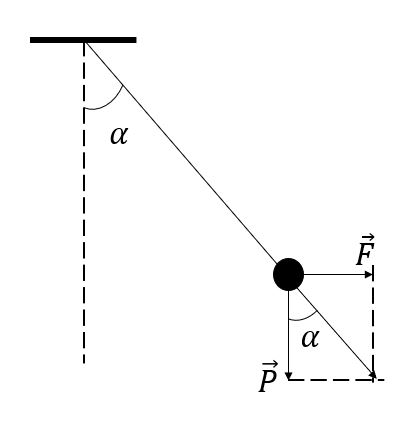
\includegraphics[scale=0.6]{../figs/VN12-Y21-PH-SYL-003-20.jpg}
		\end{center}
		
		Trọng lượng của quả cầu:
		\begin{equation*}
			P =mg =\text{2,5} \cdot 10^{-3}\ \text{N}.
		\end{equation*}
		Lực điện tác dụng lên quả cầu mang điện:
		\begin{equation*}
			F_\text{đ}=qE =\text{2,5} \cdot 10^{-3}\ \text{N}.
		\end{equation*}
		Từ hình vẽ ta có:
		\begin{equation*}
			\tan \alpha = \dfrac{F_\text{đ}}{P} = 1 \Rightarrow \alpha = 45^\circ.
		\end{equation*}
		
		
	}
	\item \mkstar{3}
	
	\cauhoi{Cường độ điện trường của một điện tích điểm tại A bằng 72 V/m, tại B bằng 18 V/m. Hỏi cường độ điện trường tại trung điểm M của AB là bao nhiêu? Cho biết A, B, M cùng nằm trên một đường sức.
		\begin{mcq}(4)
			\item 36 V/m.
			\item 48 V/m.
			\item 32 V/m.
			\item 35 V/m.
		\end{mcq}
	}
	
	\loigiai{\textbf{Đáp án: C.}
		
		Ta có: 
		\begin{equation*}
			E = k\dfrac{Q}{r^2} \Rightarrow \dfrac{E_\text{A}}{E_\text{B}} =\left(\dfrac {R_\text{B}}{R_\text{A}} \right)^2 \Rightarrow \dfrac {R_\text{B}}{R_\text{A}} = 2. 
		\end{equation*}
		Vì M là trung điểm của AB nên:
		\begin{equation*}
			R_\text{M} = \dfrac{R_\text{A} + R_\text{B}}{2} \Rightarrow R_\text{M} = \text{1,5} R_\text{A}.
		\end{equation*}
		Lại có:
		\begin{equation*}
			\dfrac{E_\text{M}}{E_\text{A}} =\left(\dfrac {R_\text{A}}{R_\text{M}} \right)^2 =\dfrac{4}{9} \Rightarrow E_\text{M} = 32\ \text{V/m}.
		\end{equation*}
		
	}
	\item \mkstar{3}
	
	\cauhoi{Một quả cầu nhỏ mang điện tích đang được cân bằng trong điện trường do tác dụng của trọng lực và lực điện trường. Đột ngột giảm độ lớn điện trường đi còn một nửa nhưng vẫn giữ nguyên phương và chiều của đường sức điện. Tính thời gian để quả cầu di chuyển được 5 cm trong điện trường. Lấy $g = 10\ \text{m/s}^2$.
		\begin{mcq}(4)
			\item 5 s.
			\item 2 s.
			\item 4 s.
			\item $\sqrt 2$ s.
		\end{mcq}
	}
	
	\loigiai{\textbf{Đáp án: D.}	
		
		Gọi $\vec{F}_1,\vec{F}_2$ là lực điện trường lúc đầu và sau.
		
		Các lực tác dụng lên quả cầu gồm trọng lực $\vec P$ và lực điện $\vec F$.
		
		Lúc đầu quả cầu đang cân bằng nên:
		\begin{equation*}
			\vec P + \vec F_1 =0 \Rightarrow mg =qE 
		\end{equation*}	
		Khi độ lớn điện trường giảm đi một nửa thì:
		\begin{equation*}
			F_2 = \dfrac{qE}{2} =\dfrac{mg}{2}.
		\end{equation*}	
		Biểu thức định luật II Newton là:
		\begin{equation*}
			\vec P + \vec F_2 = m\vec a.
		\end{equation*}	
		Chọn chiều dương hướng xuống
		\begin{equation*}
			\Rightarrow mg - F_2 =ma \Rightarrow a =\dfrac{g}{2} =5\ \text{m/s}^2. 
		\end{equation*}	
		Lại có:
		\begin{equation*}
			S=  \dfrac{1}{2}at^2 \Rightarrow t = \sqrt{\dfrac{2S}{a}} =\sqrt 2\ \text{s}.
		\end{equation*}	
		
		
	}
	\item \mkstar{3}
	
	\cauhoi{Tại ba đỉnh của một tam giác đều trong không khí, đặt ba điện tích giống nhau $q_1 =q_2 =q_3=q=6 \cdot 10^{-7}\ \text{C}$. Hỏi phải đặt điện tích $q_0$  tại đâu, có giá trị bao nhiêu để hệ điện tích cân bằng?
		\begin{mcq}
			\item Tâm của tam giác, $q_0 =- \text{3,46}\cdot 10^{-7}\ \text{C}$.
			\item Tâm của tam giác, $q_0 = \text{3,46}\cdot 10^{-7}\ \text{C}$.
			\item Tâm đường tròn ngoại tiếp tam giác, $q_0 = \text{3,46}\cdot 10^{-7}\ \text{C}$.
			\item Tâm đường tròn nội tiếp tam giác, $q_0 = \text{3,46}\cdot 10^{-7}\ \text{C}$.
		\end{mcq}
	}
	
	\loigiai{\textbf{Đáp án: A.}
		\begin{center}
			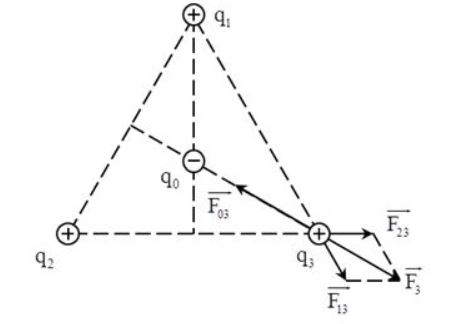
\includegraphics[scale=0.8]{../figs/VN12-Y21-PH-SYL-003-24.jpg}
		\end{center}
		
		Vì 3 điện tích $q_1, q_2, q_3$ bằng nhau, nên nếu một điện tích cân bằng thì cả ba điện tích sẽ cân bằng.
		
		Xét lực tác dụng lên điện tích $q_3$: 
		\begin{equation*}
			\vec F_3 =\vec F_{13} + \vec F_{23}.
		\end{equation*}
		
		Với 
		\begin{equation*}
			F_{13} =F_{23} = k\dfrac{q^2}{a^2} \Rightarrow F_3 =2F_{13}\cos 30^\circ=F_{13} \sqrt 3
		\end{equation*}	
		Lực $\vec F_3$ có phương là phân giác của góc C.
		
		Để $q_3$ cân bằng thì cần phải có thêm lực $\vec F_{03}$ do $q_0$ tác dụng lên $q_3$ sao cho $\vec F_3$ ngược chiều với $\vec F_{03}$ và $F_3 = F_{03} \Rightarrow q_0 <0$.
		
		Xét tương tự với $q_1, q_2, q_3$ thì $q_0$ phải nằm tại tâm của tam giác và điện tích $q_0<0$.
		
		Vậy: 
		\begin{equation*}
			F_{03} =F_3 =k \dfrac{|q_0q_3|}{\left(\dfrac{2}{3} \dfrac{a\sqrt 3}{2}\right)^2} \Rightarrow q_0 = -\text{3,46} \cdot 10^{-7}\ \text{C}.
		\end{equation*}
		
		
	}
		\item \mkstar{3}
	
	\cauhoi{Điện tích điểm $q$ di chuyển trong một điện trường đều có cường độ điện trường 800 V/m theo một đoạn thẳng AB. Đoạn AB dài 12 cm và vectơ độ dời $\overrightarrow{AB}$ hợp với đường sức điện một góc $30^\circ$. Biết công của lực điện trong sự di chuyển của điện tích $q$ là $-\text{1,33}\cdot 10^{-4}\ \text{J}$. Điện tích $q$ có giá trị bằng
		\begin{mcq}(4)
			\item $-\text{1,6} \cdot 10^{-6}\ \text{C}$.
			\item $\text{1,6} \cdot 10^{-6}\ \text{C}$.
			\item $-\text{1,4} \cdot 10^{-6}\ \text{C}$.
			\item $\text{1,4} \cdot 10^{-6}\ \text{C}$.
		\end{mcq}
	}
	
	\loigiai{\textbf{Đáp án: A.}
		
		Với 
		\begin{equation*}
			d = \text{AB} \cos 30^\circ = \text{0,06} \sqrt 3\ \text{m}.
		\end{equation*}
		Ta có: 
		\begin{equation*}
			A = qEd \Rightarrow q =\dfrac{A}{Ed} = -\text{1,6}\cdot 10^{-6}\ \text{C}
		\end{equation*}
		
		
	}
	\item \mkstar{3}
	
	\cauhoi{Một hạt bụi khối lượng $10^{-8}\ \text{g}$ mang điện tích $5\cdot 10^{-5}\ \text{C}$ chuyển động trong điện trường đều theo một đường sức điện từ điểm M đến điểm N thì vận tốc tăng từ $2\cdot 10^4 \ \text{m/s}$ đến $\text{3,6} \cdot 10^4\ \text{m/s}$. Biết đoạn đường MN dài 5 cm, cường độ điện trường đều là
		\begin{mcq}(4)
			\item 2462 V/m.
			\item 1685 V/m.
			\item 2175 V/m.
			\item 1792 V/m.
		\end{mcq}
	}
	
	\loigiai{\textbf{Đáp án: D.}
		
		Theo định lí biến thiên động năng ta có:
		\begin{equation*}
			A = W_{\text{đ}_\text{N}}-W_{\text{đ}_\text{M}} \Rightarrow \dfrac{mv^2_{\text{N}}}{2}- \dfrac{mv^2_{\text{M}}}{2} = qEd
		\end{equation*}
		\begin{equation*}
			\Rightarrow E =\dfrac{m}{2qd} (v^2_\text{N}-v^2_\text{M}) = 1792\ \text{V/m}.
		\end{equation*}
		
		
	}
	\item \mkstar{3}
	
	\cauhoi{Một electron chuyển động dọc theo đường sức của một điện trường đều. Cường độ điện trường có độ lớn bằng 100 V/m. Vận tốc ban đầu của electron là $3\cdot 10^5\ \text{m/s}$, khối lượng của electron là $\text{9,1}\cdot 10^{-31}\ \text{kg}$. Từ lúc bắt đầu chuyển động đến khi có vận tốc bằng 0 thì electron đã đi được quãng đường
		\begin{mcq}(4)
			\item 5,12 mm.
			\item 0,256 m.
			\item 5,12 m.
			\item 2,56 mm.
		\end{mcq}
	}
	
	\loigiai{\textbf{Đáp án: D.}
		
		Áp dụng bảo toàn cơ năng trong điện trường đều ta có
		
		\begin{equation*}
			qEd =-\dfrac{1}{2} mv^2_0 \Rightarrow d = \dfrac{1}{2} \dfrac{(-mv^2_0)}{qE} = \text{2,56}\ \text{mm}.
		\end{equation*}
		
	}
	\item \mkstar{3}
	
	\cauhoi{Cho một điện tích thử q di chuyển trong một điện trường đều dọc theo hai đoạn thẳng MN và NP. Biết rằng lực điện sinh công dương và MN dài hơn NP. Hỏi kết quả nào sau đây là đúng, khi so sánh các công $A_\text{MN}$ và $A_\text{NP}$ của lực điện?
		\begin{mcq}(2)
			\item $A_\text{MN} >A_\text{NP} $.
			\item $A_\text{MN} <A_\text{NP} $.
			\item $A_\text{MN} = A_\text{NP} $.
			\item Cả 3 trường hợp đều có thể xảy ra.
		\end{mcq}
	}
	
	\loigiai{\textbf{Đáp án: D.}
		
		Công của lực điện tác dụng nên điện tích q khi di chuyển trên các đoạn thẳng MN và NP được xác định bởi công thức:
		\begin{equation*}
			A_\text{MN} = qE\text{MN}\cos \alpha_\text{MN}; A_\text{NP} = qE\text{NP}\cos \alpha_\text{NP}.
		\end{equation*}
		Trong đó 
		\begin{equation*}
			A_\text{MN} > 0; A_\text{NP} > 0; q > 0; \text{MN} > \text{NP}.
		\end{equation*}
		Nhưng vì không xác định được $\cos \alpha_\text{MN}$ lớn hơn, nhỏ hơn, hay bằng $\cos \alpha_\text{NP}$ và hàm cos có thể nhận giá trị trong khoảng $[-1; 1]$ nên $A_\text{MN}$ có thể lớn hơn, nhỏ hơn, hay bằng $A_\text{NP}$ tùy theo giá trị của $\cos \alpha_\text{MN}$ và $\cos \alpha_\text{NP}$.
		
		
	}
	\item \mkstar{3}
	
	\cauhoi{Một electron được thả không vận tốc đầu ở sát bản âm, trong điện trường đều giữa hai bản kim loại phẳng, tích điện trái dấu. Cường độ điện trường giữa hai bản là 1000 V/m. Khoảng cách giữa hai bản là 1 cm. Tính động năng của electron khi nó đến đập vào bản dương.
		\begin{mcq}(4)
			\item $\text{1,6}\cdot 10^{-18}\ \text{J}$.
			\item $\text{2,6}\cdot 10^{-16}\ \text{J}$.
			\item $-\text{1,6}\cdot 10^{-18}\ \text{J}$.
			\item $\text{3,6}\cdot 10^{-18}\ \text{J}$.
		\end{mcq}
	}
	
	\loigiai{\textbf{Đáp án: A.}	
		
		Lực điện trường tác dụng lên electron (điện tích âm) có chiều ngược với chiều điện trường do đó electron di chuyển ngược chiều điện trường	
		\begin{equation*}
			\Rightarrow \alpha = (\vec E, \vec s) = 180^\circ.
		\end{equation*}
		Áp dụng định lý động năng cho sự di chuyển của electron:
		\begin{equation*}
			W_{\text{đ} (+)} - W_{\text{đ} (-)} = qEs\cos 180^\circ.
		\end{equation*}
		Động năng ban đầu tại bản (-) của electron: $W_{\text{đ} (-)} = 0$ do electron được thả không vận tốc đầu.
		
		Động năng của electron khi nó đến đập vào bản dương:
		\begin{equation*}
			W_{\text{đ} (+)} = qEs\cos 180^\circ = \text{1,6}\cdot 10^{-18}\ \text{J}.
		\end{equation*}
		
		
		
	}
	\item \mkstar{3}
	
	\cauhoi{Một electron chuyển động dọc theo đường sức của một điện trường đều. Cường độ điện trường $E = 200\ \text{V/m}$. Vận tốc ban đầu của electron là $3\cdot 10^5\ \text{m/s}$, khối lượng của elctron là $\text{9,1}\cdot 10^{-31}\ \text{kg}$. Tại lúc vận tốc bằng không thì nó đã đi được đoạn đường bao nhiêu?
		\begin{mcq}(4)
			\item 5,12 mm.
			\item 2,56 mm.
			\item 1,28 mm.
			\item 10,24 mm.
		\end{mcq}
	}
	
	\loigiai{\textbf{Đáp án: C.}
		
		Công của lực điện là 
		\begin{equation*}
			A = qEd =-e Ed =\Delta W.
		\end{equation*}
		Theo định luật bảo toàn cơ năng ta có:
		\begin{equation*}
			A = -eEd = 0 -\dfrac{mv^2}{2}
		\end{equation*}
		\begin{equation*}
			\Rightarrow d = \dfrac{mv^2}{2Ee} = \text{1,28} \cdot 10^{-3}\ \text {m} = \text{1,28}\ \text{mm}.
		\end{equation*}
		
		
	}
	\item \mkstar{4}
	
	\cauhoi{Cho hai tấm kim loại song song, nằm ngang, nhiễm điện trái dấu. Khoảng không gian giữa hai tấm kim loại đó chứa đầy dầu. Một quả cầu bằng sắt bán kính $R$ = 1 cm mang điện tích q nằm lơ lửng trong lớp dầu. Điện trường giữa hai tấm kim loại là điện trường đều hướng từ trên xuống và có độ lớn 20000 V/m. Hỏi độ lớn và dấu của điện tích q. Cho biết khối lượng riêng của sắt là 7800 kg/m$^3$, của dầu là 800 kg/m$^3$. Lấy g = 10 m/s$^2$.
		\begin{mcq}(2)
			\item $q=-\text{14,7} \cdot 10^{-6}\ \text{C}$.
			\item $q=\text{14,7} \cdot 10^{-6}\ \text{C}$.
			\item $q=-\text{1,8} \cdot 10^{-6}\ \text{C}$.
			\item $q=\text{1,8} \cdot 10^{-6}\ \text{C}$.
		\end{mcq}
	}
	
	\loigiai{\textbf{Đáp án: A.}
		
		Cho các lực tác dụng lên quả cầu gồm: lực điện $\vec F$, trọng lực $\vec P$ hướng xuống và lực đẩy Acsimet $\vec F_\text{A}$	hướng lên. Điều kiện cân bằng của quả cầu:
		\begin{equation*}
			\vec P + \vec F_\text{đ} + \vec F_\text{A} = 0.
		\end{equation*}
		Lại có:
		\begin{equation*}
			P=mg = \rho_\text{vật} Vg = \rho_\text{vật} \dfrac{4}{3} \pi R^3 g.
		\end{equation*}
		\begin{equation*}
			F_\text{A} =  \rho_\text{mt} Vg = \rho_\text{mt} \dfrac{4}{3}R^3 g.
		\end{equation*}
		Vì khối lượng riêng của vật lớn hơn
		\begin{equation*}
			\Rightarrow P>F_\text{A} \Rightarrow F_\text{A} + F = P \Rightarrow F = P - F_\text{A}
		\end{equation*}
		\begin{equation*}
			\Leftrightarrow |q|E =P- F_\text{A} \Rightarrow |q| =\dfrac{P-F_\text{A}}{E} = \text{14,7} \cdot 10^{-6}\ \text{C}.
		\end{equation*}
		Vậy để vật cân bằng thì lực điện phải hướng lên. Lực điện ngược hướng $\vec E$.
		
		Suy ra $q<0 \Rightarrow q =-\text{14,7} \cdot 10^{-6}\ \text{C}$.
		
		
	}
	\item \mkstar{4}
	
	\cauhoi{Hai quả cầu nhỏ A và B mang những điện tích lần lượt $-2\cdot 10^{-9}\ \text{C}$ và $2\cdot 10^{-9}\ \text{C}$ được treo ở đầu hai sợi dây tơ cách điện dài bằng nhau. Hai điểm treo dây M và N cách nhau 2 cm; khi cân bằng, vị trí các dây treo có dạng như hình vẽ. Hỏi để đưa các dây treo trở về vị trí thẳng đứng người ta phải dùng một điện trường đều có hướng nào và độ lớn bao nhiêu?
		\begin{center}
			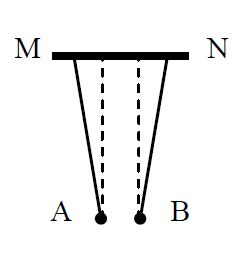
\includegraphics[scale=0.7]{../figs/VN12-Y21-PH-SYL-003-21.jpg}
		\end{center}
		\begin{mcq}
			\item Nằm ngang hướng sang phải, $E = \text{1,5} \cdot 10^4\ \text{V/m}$.
			\item Nằm ngang hướng sang trái, $E = 3 \cdot 10^4\ \text{V/m}$.
			\item Nằm ngang hướng sang phải, $E = \text{4,5} \cdot 10^4\ \text{V/m}$.
			\item Nằm ngang hướng sang phải, $E = \text{3,5} \cdot 10^4\ \text{V/m}$.
		\end{mcq}
	}
	
	\loigiai{\textbf{Đáp án: C.}
		
		\begin{center}
			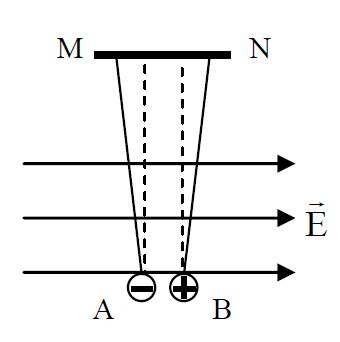
\includegraphics[scale=0.6]{../figs/VN12-Y21-PH-SYL-003-22.jpg}
		\end{center}
		Để đưa các dây treo trở về vị trí thẳng đứng cần phải tác dụng lực điện trường ngược chiều với lực tĩnh điện và cùng độ lớn với lực tĩnh điện: $F'=F$.
		
		Với quả cầu A: 
		\begin{equation*}
			|q|E =k\dfrac{q^2}{\text{AB}^2}.
		\end{equation*}
		Suy ra:
		\begin{equation*}
			E =k\dfrac{|q|}{\text{AB}^2} =k \dfrac{|q|}{\text{MN}^2} = \text{4,5} \cdot 10^4\ \text{V/m}.
		\end{equation*}
		Và vì điện tích treo tại A là điện tích âm nên $\vec E$ ngược chiều với $\vec{F}'$ nghĩa là cùng chiều với $\vec F$ (hướng từ trái sang phải).
		
		Với quả cầu B: tương tự.
		
		Vậy: để đưa các dây treo trở về vị trí thẳng đứng cần phải dùng một điện trường đều có hướng từ trái sang phải và độ lớn $E = \text{4,5} \cdot 10^4\ \text{V/m}$. 
		
		
	}
	\item \mkstar{4}
	
	\cauhoi{Một hòn bi nhỏ bằng kim loại được đặt trong dầu. Bi có thể tích $V = 10\ \text{mm}^3$, khối lượng $m = 9\cdot 10^{-5}\ \text{kg}$. Dầu có khối lượng riêng $D = 800\ \text{kg/m}^3$. Tất cả được đặt trong một điện trường đều, $\vec E$ hướng thẳng đứng từ trên xuống, $E = \text{4,1}\cdot 10^5\ \text{V/m}$. Tìm điện tích của bi để nó cân bằng lơ lửng trong dầu. Cho $g = 10\ \text{m/s}^2$.
		
		\begin{mcq}(4)
			\item - 1 nC.
			\item 1,5 nC.
			\item - 2 nC.
			\item 2,5 nC.
		\end{mcq}
	}
	
	\loigiai{\textbf{Đáp án: C.}
		
		\begin{center}
			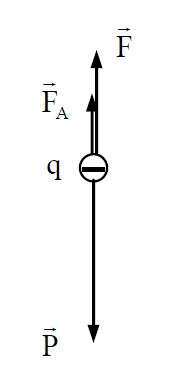
\includegraphics[scale=0.7]{../figs/VN12-Y21-PH-SYL-003-23.jpg}
		\end{center}
		Các lực tác dụng lên hòn bi:
		
		- Trọng lực
		\begin{equation*}
			\vec P =m\vec g \ \text{(hướng xuống)}.
		\end{equation*}
		- Lực đẩy Acsimet 
		\begin{equation*}
			\vec F_\text{A} = - DV\vec g\ \text{(hướng lên)}.
		\end{equation*}
		- Lực điện trường 
		\begin{equation*}
			\vec F =q\vec E.
		\end{equation*}
		(hướng xuống nếu $q>0$; hướng lên nếu $q<0$).
		
		Hòn bi nằm cân bằng (lơ lửng) khi: 
		\begin{equation*}
			\vec P + \vec F_\text{A} +F =0 \Leftrightarrow \vec P' + F =0.
		\end{equation*}
		Vì $P>F_\text{A}$ nên $P' = P-F_\text{A} \Rightarrow \vec F$ phải hướng lên.
		
		Mà $q<0$ và $P' = P-F_\text{A}$.
		\begin{equation*}
			\Rightarrow |q|E =mg -DVg
		\end{equation*} 		
		\begin{equation*}
			\Rightarrow |q|  = \dfrac{|mg - DVg|}{E} = 2\cdot 10^{-9}\ \text{C}.
		\end{equation*}
		Vì $q<0$ nên $q = -2 \cdot 10^{-9}\ \text{C}$.
		
		
		
	}
	



	\item \mkstar{4}
	
	\cauhoi{Một điện tích $q = 4\cdot 10^{-8}\ \text{C}$ di chuyển trong một điện trường đều có cường độ điện trường $E = 100\ \text{V/m}$ theo một đường gấp khúc ABC. Đoạn AB dài 20 cm và vectơ độ dời $\vec{AB}$ làm với các đường sức điện một góc $30^\circ$. Đoạn BC dài 40 cm và vectơ độ dời $\vec{BC}$ làm với các đường sức điện một góc $120^\circ$. Tính công của lực điện.
		\begin{mcq}(4)
			\item $\text{0,108}\cdot 10^{-6}\ \text{J}$.
			\item $-\text{0,108}\cdot 10^{-6}\ \text{J}$.
			\item $\text{1,492}\cdot 10^{-6}\ \text{J}$.
			\item $-\text{1,492}\cdot 10^{-6}\ \text{J}$.
		\end{mcq}
	}
	
	\loigiai{\textbf{Đáp án: B.}
		
		Công của lực điện trường trên đường gấp khúc ABC là
		\begin{equation*}
			A_\text{ABC} = A_\text{AB} + A_\text{BC} = qEd_1 + qEd_2 
		\end{equation*}
		\begin{equation*}
			= qE\text{AB} \cos 30^\circ + qE\text{BC} \cos 120^\circ = - \text{0,108} \cdot 10^{-6}\ \text{J}.
		\end{equation*}
		
		
	}







\end{enumerate}

\whiteBGstarEnd

\loigiai{\begin{center}
		\textbf{BẢNG ĐÁP ÁN}
	\end{center}
	\begin{center}	
		\begin{tabular}{|m{2.8em}|m{2.8em}|m{2.8em}|m{2.8em}|m{2.8em}|m{2.8em}|m{2.8em}|m{2.8em}|m{2.8em}|m{2.8em}|}
			\hline
			1. B & 2. C & 3. B & 4. D & 5. B & 6. D  & 7. B & 8. D & 9. D & 10. C \\
			\hline
			11. D & 12. C & 13. B & 14. A & 15. C & 16. B & 17. D & 18. A & 19. B & 20. A \\
			\hline
			21. C & 22. A & 23. C & 24. A & 25. C & 26. D & 27. B & 28. C & 29. D & 30. A \\
			\hline
			31. A & 32. D & 33. D & 34. D & 35. A & 36. C & 37. A & 38. C & 39. C & 40. B \\
			\hline
		\end{tabular}
\end{center}}